\section{Einleitung}
In Rahmen dieses Praktikums soll ein flexibler Klassifikator erstellt werden, der Teilchen abhängig von ihrem Bewegungsverlauf zu einer der vorgegebenen Klassen zuordnet. Hierfür werden Trainingsdaten der Bewegung realer Schüttgutteilchen zur Verfügung gestellt. Teilchen unterschiedlichen sich hierbei nicht nur durch ihren auf dem Band zurückgelegten Pfad, sondern auch hinsichtlich der Geschwindigkeit in Bandrichtung und orthogonal zur Bandrichtung.

\subsection{Aufbau}

\begin{figure}[!h]
    \centering
    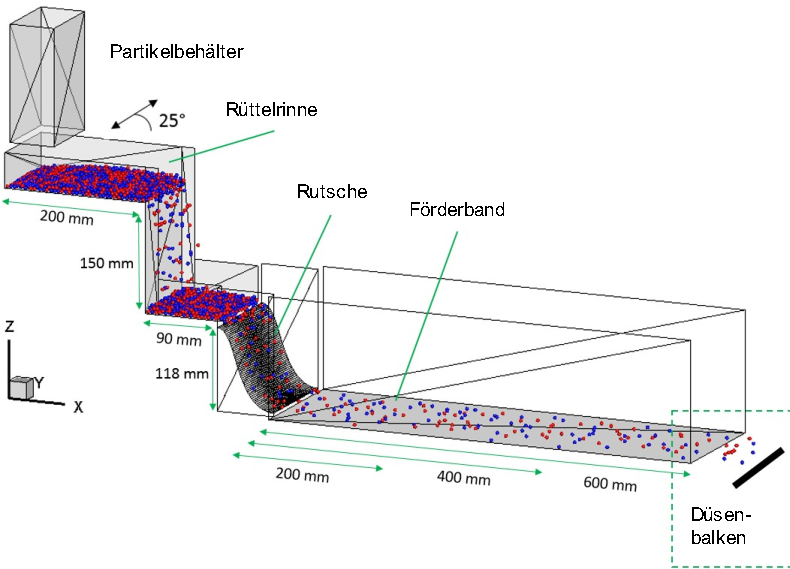
\includegraphics[width=0.7\textwidth]{pics/aufbau.pdf}
    \caption{Aufbau \cite{ITM07_BrunnSawo}}
    \label{fig:Aufbau}
\end{figure}